\documentclass{article}
\usepackage{amsmath, amssymb,amsfonts,tikz, mdframed}
\usetikzlibrary{shapes,arrows,calc,positioning,backgrounds}
\title{Algorithms \& Complexity: Lecture 4, Hierarchy theorems and a complexity zoo}
\author{Sam Barrett}

\newcommand{\T}{\texttt{T }}
\newcommand{\True}{\texttt{True }}
\newcommand{\F}{\texttt{F }}
\newcommand{\False}{\texttt{False }}
\newcommand{\NP}{\mathbf{NP}}
\renewcommand{\P}{\mathbf{P}}
\newcommand{\N}{\mathbb{N}}

\newmdtheoremenv{lemma}{Lemma}
\newmdtheoremenv{definition}{Definition}
\newmdtheoremenv{theorem}{Theorem}

\begin{document}
\maketitle

\section{Low-level conventions}
\label{sec:conventions}

\subsection{Representation of Turing machines}
\label{subsec:representingTMs}
\begin{itemize}
  \item We will associate with every $\alpha\in \{ 0,1 \} ^{*}$ a Turing machine $M_{\alpha}$ s.t. for each Turing machine $M$, there are \textbf{infinitely many} $\alpha$ where $M = M_{\alpha}$.

        We will also fix a \textbf{bijection} between $\{ 00,11 \} ^{*}$ (a fragment of all binary strings) and the set of all TMs (for every word inside this language, there is a corresponding unique TM), we will write $M_{\beta}$ for the TM $M$ that $\beta \in \{ 00,11 \} ^{*}$ is mapped to. Here $\beta$ is the canonical description of $M$ or a \textit{code of $M$} .

  \item We will extend our notion of $M_{\beta}$ to $\alpha \in \{ 0,1 \} ^{*}$ (any binary string), we may write $\alpha = \beta\gamma$ with $\beta \in \{ 00,11 \} ^{*}$ and with $\gamma \in \{ 0,1 \} ^{*}$ being either empty or beginning with 01 or 10. In this case we also set $M_{\alpha} := M_{\beta}$. Here $\alpha$ is a \textbf{description} of $M = M_{\beta}$.

        Unpacking this:

        If we have a bitstring \(\alpha\) and want to find the machine that it represents, you write \(\alpha\) in the form \(\beta\gamma\) and extract the initial \(\beta\) section.
\end{itemize}

A very useful property of the above framework is that given any \(\alpha = \beta\gamma\) we can \textbf{computably extract} low-level information about $M = M_{\alpha}$ such as its states, transition table, alphabet etc. Extracting this information can be done in time and space \textbf{only dependant on \(\beta\)}, its canonical description. We can completely ignore \(\gamma\) in this case, thinking of it as \textit{padding}.

\textbf{Note:} we know when to stop reading \(\beta\) as we treat the \textit{gadgets} ``01'' or ``10'' as blanks/ end of input markers.

\subsection{Constructable functions}

We shall identify $\N$ and $\{ 0,1 \} ^{*}$ by some \textit{fixed bijective coding} . This will make more sense later in the lecture. Refer back.

\subsubsection{Time-constructibility convention}

All functions $t: \N \rightarrow \N $ we consider are \textbf{time-constructible} meaning:
\begin{itemize}
  \item $t(n) \geq n$
  \item There is a TM $M$ computing $1^{n} \mapsto t(n)$ in time $t(n)$
\end{itemize}

\subsubsection{Space-constructibility convention}

All functions $s : \N \rightarrow \N$ we consider are \textbf{space-constructible} meaning:
\begin{itemize}
  \item $s(n) \geq\log n$
        \item There is a TM $M$ computing $1^{n} \mapsto s(n)$ in space $O(s(n))$
\end{itemize}

\section{Universality}
\label{sec:universality}

We have previously seen the following:

\subsection{Normal form of Turing machines}
\label{subsec:TMNF}

\begin{theorem}\label{theorem:U}
  Suppose $M$ computes $f : \{ 0,1 \}^* \rightarrow \{ 0,1 \}$ in time $t(n)$ and space $s(n)$. Where $M$ can have an arbitrary alphabet and any number of tapes.

  There exists a 3-tape TM $\tilde{M}$ with alphabet $\{ \rhd, \Box, 0,1 \} $ computing $f$,
  \begin{itemize}
    \item in time $O(t(n)^{2})$
    \item in space $O(s(n))$
  \end{itemize}

  These constraints depend on $M$ and not its description \(\tilde{\beta}\)

  Moreover, we can compute the canonical description \(\tilde{\beta}\) of $\tilde{M}$ from the canonical description \(\beta\) of $M$ or any other description,\(\alpha\), of $M$ for that matter (in the form \(\alpha=\beta\gamma\)).
\end{theorem}

\subsection{An efficient universal machine, $\mathcal{U}$}
\label{subsec:uni-M}

For a TM $M$ and a bitstring $x \in \{ 0,1 \}^*$, we shall write $M(x) \in \{ 0,1 \}^* \cup \{ \uparrow \} $ for the output of $M$ on $x$, if it exists, otherwise $\uparrow$ if it diverges or does not terminate.

\begin{theorem}
  There exists a TM $\mathcal{U}$ s.t. $\forall x \in \{ 0,1 \}^*$ and $\alpha \in \{ 0,1 \}^*$, we have $\mathcal{U}(x,\alpha) = M_{\alpha}(x)$

  Moreover, we can also talk about its complexity, if $M_{\alpha}$ halts on $x$ in $t$ steps and uses $s$ space, then $\mathcal{U}$ halts on $(x,\alpha)$ within $c_{M}t^{2}$ steps and $d_{M}s$ space, where $c_{M}$ and $d_{M}$ are constants depending only on $M = M_{\alpha}$, \textbf{not} its description \(\alpha\). (It will precisely depend on the canonical description of $M$ \(\beta\))

  Our formulation of $\mathcal{U}$ will have \textbf{5 tapes}: 1 input and 4 work tapes.
\end{theorem}

We will now examine how $\mathcal{U}$ operates over an input $(x,\alpha)$:

\begin{enumerate}
  \item \underline{Computing the normal form}

        Let $\alpha = \beta\gamma$ be as defined in Section~\ref{subsec:representingTMs} and recall the definition of $\tilde{\beta}$ and $\tilde{M}$ from Theorem~\ref{theorem:U}

        \begin{itemize}
          \item $\mathcal{U}$ first computes $\tilde{\beta}$ from \(\alpha=\beta\gamma\) and prints it onto tape 2, it only reads up to end of \(\beta\)
          \item The first step concludes by printing a description of the start state of $M$ on tape 3
        \end{itemize}
        This step takes time and space complexity depending on \(\beta\), ignoring \(\gamma\).

        \underline{Usage of tapes and space complexity}
        \begin{itemize}
          \item From this stage onward, only the initial $x$ section of the input $(x,\alpha)$ will be used on tape 1.

                Where we can visualise our input tape as:

        \begin{center}
          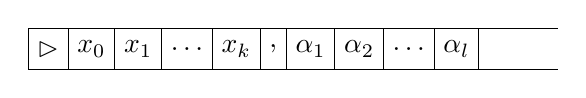
\begin{tikzpicture}[every node/.style={block},
          block/.style={minimum height=1.5em,outer sep=0pt,draw,rectangle,node distance=0pt}]


                \node (A) {$\rhd$};
                \node (B) [right = of A] {$x_{0}$};
                \node (C) [right = of B] {$x_{1}$};
                \node (D) [right = of C] {$\ldots$};
                \node (E) [right = of D] {$x_{k}$};
                \node (F) [right = of E] {,};
                \node (G) [right = of F] {$\alpha_{1}$};
                \node (H) [right = of G] {\(\alpha_{2}\)};
                \node (I) [right = of H] {$\ldots$};
                \node (J) [right = of I] {\(\alpha_{l}\)};

                \draw (J.north east) -- ++(1cm,0) (J.south east) -- ++ (1cm,0);
              \end{tikzpicture}
            \end{center}

                Where the comma can be encoded as the first occurrence of our 01 or 10 gadget and our delimiter, if we encode our $x$ in the same way as we do for our canonical descriptions \(\beta\).


          \item Tape 2 will become \textbf{read-only} and is used as a \textit{lookup} table for simulating the transitions of $\tilde{M}$. Therefore, this tape uses space $\tilde{|\beta|}$

          \item Tape 3 will always store a \textit{current state}, using only as much space as the description of a state of $\tilde{M}$ (without loss in generality our space usage is $< | \tilde{\beta} | $)

                \item Tapes 4 \& 5 will be used as the two work tapes of $\tilde{M}$. Therefore, these tapes use only as much space as $M$ does on its work tapes.

        \end{itemize}

  \item \underline{The simulation \& time complexity}

        Each step of $\tilde{M}$ is simulated as follows:

        \begin{itemize}
          \item $\mathcal{U} $ inspects tape 3 to find the current state $q$ and reads the symbols $b_{1},b_{4}, b_{5}$ at the head-positions of tapes 1,4 and 5. This process takes no (0) time.
          \item $\mathcal{U}$ scans the transition table of $\tilde{M}$ (by inspecting tape 2) to find the transition corresponding to $(q,b_{1}, b_{4}, b_{5})$. The time of this depends only on $\tilde{\beta}$
          \item $\mathcal{U}$ overwrites tape 3 with the description of the new state. The time this takes depends only on $\tilde{\beta}$.
                \item $\mathcal{U}$ writes the appropriate symbols at the head-positions of tapes 4 and 5 before moving the heads of tapes 1,4 and 5 in the appropriate directions. This takes a single (1) time step.
        \end{itemize}

        $\mathcal{U}$ will halt whenever $\tilde{M}$ does, outputting the content of tape 5.

\end{enumerate}

\section{Diagonalisation}
\label{sec:diagonalisation}

\begin{theorem}(Time hierarchy theorem)
  There is a language $L\in \mathbf{\mathbf{DTIME}}(t(n)^{4})$ s.t. $L \notin \mathbf{\mathbf{DTIME}}$

  i.e. $\mathbf{DTIME}(t(n)) \subsetneq \mathbf{DTIME}(t(n)^{4})$ (one is \textbf{strictly contained within the other})

  Where $t$ is arbitrary but time constructable as defined in Section~\ref{sec:conventions}.
\end{theorem}

\subsection{Time-sensitive diagonalisation}
\label{subsec:ts-diagonalisation}

To perform diagonalisation in such a way as to concern ourselves with time complexity, we define a Turing machine $D$ that does the following:
\begin{definition}(Turing machine $D$)
  \label{def:D}
\begin{itemize}
  \item on input $x$ ($x$ is a binary string $x \in \{ 0,1 \}^*$), run $\mathcal{U}$ on $(x,x)$ for $t(|x|)^{3}$ steps, we use $t(|x|)^{3}$ as it is somewhere between the time overhead for $\mathcal{U}$ ($t(n)^{2}$) and our states time hierarchy constraint of $t(n)^{4}$.
  \item if it halts in this time and rejects (where rejecting means it outputs 0) then accept (output 1)
  \item otherwise, reject (output 0).
\end{itemize}

\end{definition}

We can now define a language $L \subseteq \{ 0,1 \}^*$ as the language that is decided by $D$. $L$ is just the set of descriptions of Turing machines for which when $\mathcal{U}$ runs it on itself it rejects the appropriate amount of time.

By our construction of $L$ we can observe that $L \in \mathbf{DTIME}(t(n)^{4})$ as our machine $D$ can only run for $t(|x|)^{3}$ steps.

We claim therefore, that $L$ is the \textbf{explicit} language that separates $\mathbf{DTIME}(t(n^{4}))$ from $\mathbf{DTIME}(t(n))$, meaning that $L \notin \mathbf{DTIME}(t(n))$. We will prove this by contradiction.

\subsubsection{Proof}

Assume that $L \in \mathbf{DTIME}(t(n))$, and suppose $M$ decides $L$ taking $ct(n)$ steps on inputs of length $n$.

We now use $\mathcal{U}$ to simulate $M$ and say it does this within $c_{M}ct(n)^{2}$ steps on inputs of length $n$. Where $c_{M}$ depends only on $M$ and not its description.

Let us fix $n_{0} \in \N$ s.t. if $n \geq n_{0}$ then $t(n)^{3} > c_{M}ct(n)^{2}$.

This is a key point, it means that there is a point in $\N$, $n_{0}$ where whenever $n$ is greater than $n_{0}$ we can say that $t(n)^{3}$ (the number of steps $\mathcal{U}$ runs for) is greater than the number of steps our machine $M$ is purported to take.

This is where \textit{``foo is dependant only on bar not its description''} becomes important, the trick to \textit{breaking} this inequality and deriving a contradiction is to let \(\alpha\) be a description of $M$ (which has infinitely many descriptions) with $|\alpha| \geq n_{0}$

We will now examine what happens when we run $D$ with the input \(\alpha\) that I described above.

\begin{itemize}
  \item $D$ runs $\mathcal{U}$ on $(\alpha,\alpha)$ for $t(|\alpha|)^{3}$ steps as per our definition of $D$ in Definition~\ref{def:D}
  \item From our fixing above, along with our definition of \(\alpha\), we can say that $t(|\alpha|)^{3} \geq c_{M}ct(|\alpha|)^{2}$, giving us in turn:

        \[
        \mathcal{U}(\alpha,\alpha) = M_{\alpha}(\alpha) = M(\alpha)
        \]

        As $M$ must halt on \(\alpha\) \textbf{within} $ct(|\alpha|)$ steps, by our assumption of $M$.

  \item As per our definition of $D$, as $M(\alpha)$ halts, $D$ must return $1-M(\alpha)$ as it always returns the inverse.

        However, by doing so, as $M$ was meant to decide the language described by $D$ we have derived a contradiction by constructing a situation in which $M$ and $D$ disagree on an input \(\alpha\). Therefore, $M$ could \textbf{not} have decided the language described by $D$.
\end{itemize}

By a similar proof, tracking space instead of time we can show that:

\begin{theorem}(Space hierarchy theorem)
  There is a language $L \in \mathbf{SPACE}(t(n)^{2})$ s.t. $L\notin \mathbf{SPACE}(t(n))$
\end{theorem}

We will not go on to prove this.

\section{Consequences and the complexity \textit{zoo} }

\subsection{Separations of complexity classes}
\label{subsec:separations}

\begin{theorem}
  We have the following:

  $\bf P \subsetneq EXP$

  $\mathbf{L} \subsetneq \mathbf{PSPACE}$
\end{theorem}

\subsubsection{Proof}

For both of the above statements, the $\subseteq$ case is \textit{obvious}. However, for non-equality we have,

\[
  \mathbf{P} \subseteq \overbrace{\mathbf{DTIME}(2^{n}) \subsetneq \mathbf{DTIME}(2^{4n})}^{\text{Time hierarchy theorem}} \subseteq \mathbf{EXP}
\]

This can be seen by the time-hierarchy theorem explored earlier.

We also have for space:

\[
  \mathbf{L} \subseteq \mathbf{SPACE}(n) \subsetneq \mathbf{SPACE}(n^{2}) \subseteq \mathbf{PSPACE}
\]

which can equally be seen via the space-hierarchy theorem.


We now have a \textit{zoo} of complexity classes:

\[
  \mathbf{L} \underbrace{\subseteq}_{\text{Lecture 2}} \mathbf{P} \underbrace{\subseteq}_{\text{obv}} \mathbf{NP} \subseteq \overbrace{\mathbf{PSPACE} \underbrace{\subseteq}_{\text{obv}}\mathbf{NPSPACE}}^{ \leftarrow \text{Savitch's theorem}} \subseteq \mathbf{EXP}
\]

This is all we know! Every other such problem remains open.

\end{document}
